\documentclass[a4paper,12pt]{article}
\usepackage[T2A]{fontenc}
\usepackage[utf8]{inputenc}
\usepackage[russian]{babel}
\usepackage{cmap}
\usepackage[left=15mm,right=15mm,top=15mm,bottom=20mm]{geometry}
\usepackage{amsmath}
\usepackage{amssymb}
\usepackage{graphicx}
\usepackage{caption}
\usepackage{tabularx}
\usepackage{wrapfig}
\usepackage{mathtext}



\setlength{\parindent}{10mm}
\setlength{\parskip}{2mm}
\begin{document}

        \section*{Механика}
		\subsection*{Кинематика}
		Механическим движением тела называется \textit{изменение с течением времени его 
		положения по отношению к другим телам}.

		Раздел механики, в котором движения изучаются без исследования причин, их 
		вызывающих, называют \textit{кинематикой}.

		\textit{Всякое движение, а также покой тела (как частный случай движения) 
		относительны}.

		Тела, относительно которых рассматривается данное движение, называют \textit{системой 
		отчета}.

		При движении тела каждая его точка описывает некоторую линию - \textit{траекторию 
		движения}. Так как движение относительно, то \textit{траектория может зависеть от 
		выбора системы отсчета}.

		Движение тела при котором все точки тела движутся одинаково, описывая одинаковые
		траектории называется \textit{поступательным}. При поступательном движении любая
		прямая, проведенная в теле, остается параллельной самой себе.

		При \textit{вращательном движении} все точки тела движутся по окружностям, центры
		которых лежат на прямой (\textit{оси вращения}). Точки тела, лежащие на оси вращения,
		остаются неподвижными.

		В ряде случаев описание движения тела сводится к описанию движения точки.
		Если траектория движения - прямая линия, то движение точки называют 
		\textit{прямолинейным}, если траектория - кривая линия,  то движение называют
		\textit{криволинейным}.
		
		Пусть точка в своем движении перешла из точки $A$ в точку $B$. Отрезок $AB$, 
		идущий от начальной точки к конечной, называется \textit{перемещением} точки.
		Перемещение точки является \textit{вектором}.

		Пройденное точкой расстояние, отсчитанное вдоль траектории, называется 
		\textit{путем}. Путь, обозначаемый буквой $s$, всегда выражается положительным
		числом.

		Промежуток времени обозначают буквой $t$.

		Движение, при котором тело проходит за любые равные промежутки времени одинаковые
		пути, называется \textit{равномерным}.

		\textit{Скоростью равномерного движения называют отношение пути, пройденного 
		телом, к промежутку времени, за который этот путь пройден}:

		\begin{equation}
			\label{eq:f1}
			\vec{v} = s/t
		\end{equation}

		Пусть в момент времени $t_1$, считая от начального момента, тело находилось в
		точке с координатой $x_1$, а в более поздний момент $t_2$ - в точке с 
		координатой $x_2$. Разность $t_2-t_1$ дает промежуток времени $t$, в течение
		которого двигалось тело. Абсолютное значение разности $x_2-x_1$ равно 
		пройденному телом пути $s$. Формулу \ref{eq:f1} можно представить:

		\begin{equation}
			\label{eq:f2}
			\vec{v} = \frac{x_2-x_1}{t_2-t_1}
		\end{equation}


		Разность координат может быть положительной (при $x_2>x_1$), так и 
		отрицательной (при $x_1<x_2$). Знак зависит от направления в котором
		движется тело.
		
		\textit{За единицу скорости принимают скорость такого равномерного движения,
		при котором за единицу времени тело проходит путь, равный единице.}

		\begin{equation*}
			1[\text{км/ч}] = \frac{1}{3.6}[\text{м/с}]
		\end{equation*}

		\begin{wrapfigure}{l}{0.47\textwidth} % r = right
            \vspace{-10pt}
            \centering
            % 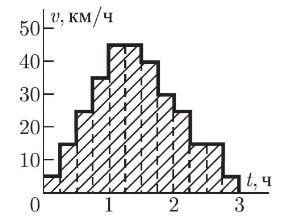
\includegraphics[width=0.46\textwidth]{01}
            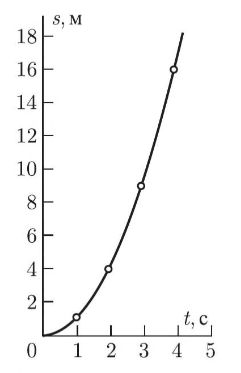
\includegraphics[scale=0.70]{02}
            \caption{График скорости}
            \label{fig:01}
        \end{wrapfigure}

		\vspace{3pt}
		Путь, пройденный за какой-либо промежуток времени, численно
		выражается площадью, ограниченной осью времени, графиком 
		скорости и двумя вертикальными отрезками, проведенными из точек,
		соответствующих началу и концу данного промежутка времени (рис.~\ref{fig:01}).

        \textit{Средней скоростью неравномерного движения на данном участке пути называют отношение 
        длины этого участка к промежутку времени, за который этот участок пройден:}

        \begin{equation}
            v_{\text{ср}} = s/t
        \end{equation}

        Если средняя скорость известна за отдельные последовательные промежутки времени,
        то можно найти среднюю скорость и за суммарное время движения.
        
        \begin{equation}
            v_{\text{ср}} = \frac{v_{1}t_{1}+v_{2}t_{2}+v_{3}t_{3}+\dots}{t_{1}+t_{2}+t_{3}+\dots}
        \end{equation}

		Среднюю скорость, измеренную за столь малый промежуток времени, что в течение этого промежутка 
		движение представляется для наших приборов равномер­ным, называю \textit{мгновенной  скоростью}.

        \begin{wrapfigure}{l}{0.47\textwidth} % r = right
            \vspace{-2pt}
            \centering
            % 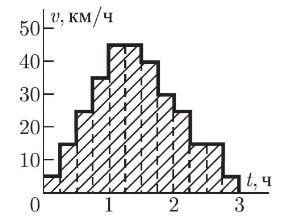
\includegraphics[width=0.46\textwidth]{01}
            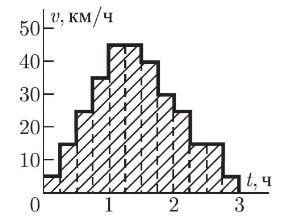
\includegraphics[scale=0.55]{01}
            \caption{График --- плавная линия}
            \label{fig:02}
        \end{wrapfigure}
            
        \vspace{0pt}
		Мгновенная скорость равномерного движения постоянна.

        Мгновенная скорость неравномерного движения величина переменная, принимающая
        различные значения в разные моменты времени. Мгновенную скорость можно считать
        изменяющейся во все время движения непрерывно, так что график пути можно изобразить
        плавной линией (рис.~\ref{fig:02}).

        Если мгно­венная скорость движущегося тела растет, то движение на­зывают \textit{ускоренным};
        если мгновенная скорость уменьшает­ся, то движение называют \textit{замедленным}.
        \textit{Равноускоренное движение} - движение в котором мгновенная скорость за любые
        равные промежутки времени увеличивается на одну и ту же величину.

        \textit{В случае равноускоренного движенuя ускорением называ­ют отношение nрuращенuя 
        скорости к nромежутку вре­мени, за который это nрuращенuе произошло:}

        \begin{equation}
			\label{eq:f5}
            \vec{a} = \frac{\vec{v}_2-\vec{v}_1}{t_2-t_1} = \frac{\vec{v}_2-\vec{v}_1}{t} \; [\text{м/с}^2]
        \end{equation}

		В случае \textit{равнозамедленного} движения ускорение оказывается отрицательным 
		(т.к. $v_2<v_1$).

		В случае ускоренного движения направления векторов скорости и ускорения одинаковы;
		в случае замедленного движения векторы скорости и ускорения направленны в противоположные
		стороны.

        Можно сказать, что ускоре­ние есть скорость изменения скорости.

        Из формулы \ref{eq:f5} находим формулу для скорости, где $v_0$ - начальная скорость:

		\begin{equation}
			\vec{v} = \vec{v}_0 + \vec{a}t
		\end{equation}

		Формула пути для равноускоренного или равнозамедленного движения:

		\begin{equation}
			s = \vec{v}_0t + \frac{\vec{a}t^2}{2}
		\end{equation}

		\begin{wrapfigure}{l}{0.5\textwidth}
			\vspace{-16pt}
			\centering
			\begin{minipage}{0.4\linewidth}
				\centering
				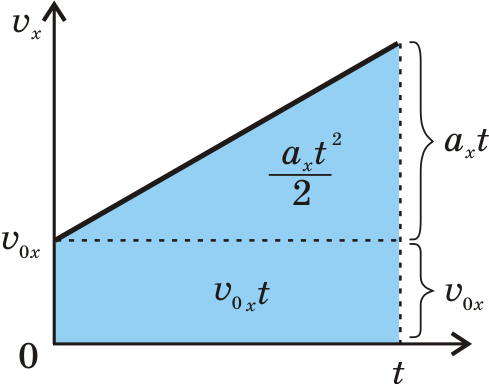
\includegraphics[width=\linewidth]{03}
				\captionof{figure}{График скорости}
				\label{fig:03}
			\end{minipage}
			\hfill
			\begin{minipage}{0.4\linewidth}
				\centering
				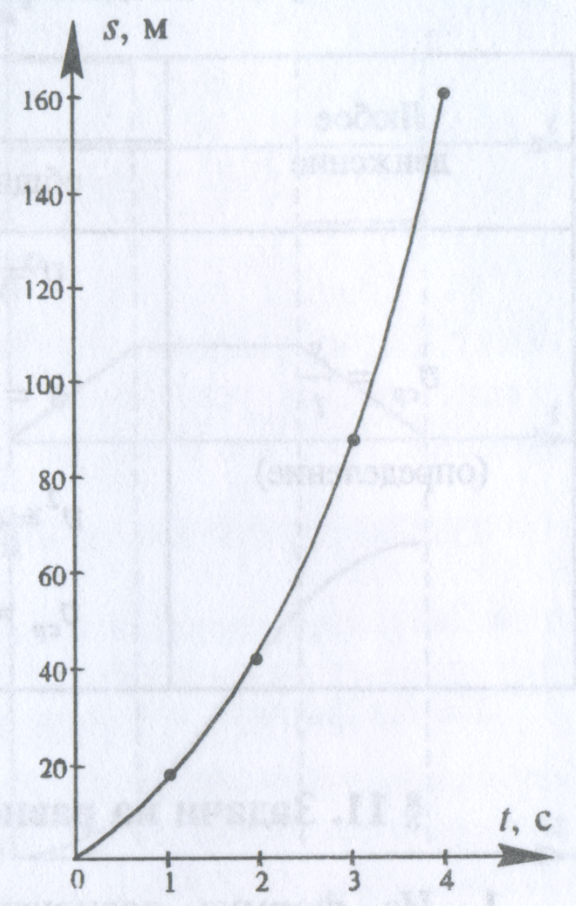
\includegraphics[width=\linewidth]{04}
				\captionof{figure}{График пути}
				\label{fig:04}
			\end{minipage}
		\end{wrapfigure}
            
        \vspace{20pt}
        Графическое представление формулы пути (рис.~\ref{fig:03}) 
		и график пути равноускоренного движения (рис.~\ref{fig:04}).

		Если начальная скорость $v_0$ равна нулю, можно выразить путь
		$s$, пройденный к моменту $t$, через скорость $v$ в этот момент
		или скорость - через пройденный путь. 
		
		В этом случае $v=at$ и $s=at^2/2$.

		Из этого следует:
		\begin{equation}
			s=\frac{\vec{v}^2}{2\vec{a}}
		\end{equation}

		\begin{equation}
			\vec{v} = \sqrt{2\vec{a}s}
		\end{equation}

		Если начальная скорость не равна нулю, то скорость в конце движения:

		\begin{equation}
			\vec{v} = \vec{v}_0 + \vec{a}t
		\end{equation}

		Следовательно:

		\begin{equation}
			s = \frac{\vec{v}^2 - \vec{v}_0^2}{2\vec{a}}
		\end{equation}

		\

		\textit{Величины, которые характеризуются числовым значением и 
		направлением в пространстве, называются векторами}.

		Числовое значение вектора называется \textit{модулем}. Модуль 
		вектора всегда положительный.

		Величины, которые характеризуются числовым значением, но которым 
		нельзя приписать направления  в  пространстве,  называют 
		\textit{скалярами}. 

		Скалярные величины равны друг другу, если совпадают по числовому 
		значению. Векторные величины равны друг другу, если совпадают 
		по модулю и по направлению.

		Любой вектор можно разложить на несколько векторов. Чаще всего 
		производят разложение векторов по направлениям осей какой-либо 
		прямоугольной системы координат.

        \begin{wrapfigure}{l}{0.5\textwidth} % r = right
            \vspace{-2pt}
            \centering
            % 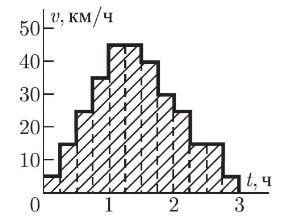
\includegraphics[width=0.46\textwidth]{01}
            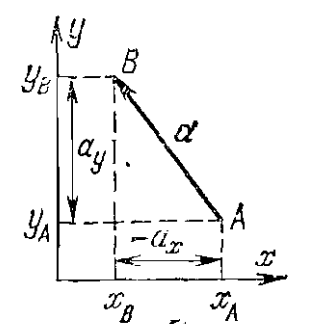
\includegraphics[scale=.9]{05}
			\captionsetup{width=0.35\textwidth}
            \caption{Проекция вектора на координатные оси}
            \label{fig:05}
        \end{wrapfigure}
            
        \vspace{0pt}
		Точка пересечения перпендикуляра с осью называется \textit{проекцией}.
        соответствующей точки (A или B) на данную ось (x или y). Разность $X_B-X_A$ 
        обозначается $a_x$ и называется проекцией вектора $a$ на ось $x$; аналогично, 
        разность $Y_B-Y_A$ обозначается $a_y$ и называется проекцией вектора $a$ 
        на ось $y$ (рис.~\ref{fig:05}).
        
        Проекции называют также компонентами вектора по координатным осям. Проекции 
        (компоненты) являются скалярами.

\end{document}